% ==========================================================================
% INFO 4617 Web Data Science -- Week 6: Parsing Static Web Pages (Chapter 6)
% Build:  latexmk -pdf slides.tex   (from this folder; no env vars needed)
% (or run `make` from the slides/ directory to build every deck)
% ==========================================================================
\documentclass[9pt,aspectratio=169]{beamer}
% Resolve the shared theme/preamble in ../common/ when compiling this
% file directly from its own folder (no TEXINPUTS needed).
\makeatletter\def\input@path{{../common/}}\makeatother
% ==========================================================================
% Shared preamble for INFO 4617 Web Data Science weekly lecture decks
% Based on the Gotham beamer theme (vendored in this directory).
% Each week's slides.tex does:  % ==========================================================================
% Shared preamble for INFO 4617 Web Data Science weekly lecture decks
% Based on the Gotham beamer theme (vendored in this directory).
% Each week's slides.tex does:  % ==========================================================================
% Shared preamble for INFO 4617 Web Data Science weekly lecture decks
% Based on the Gotham beamer theme (vendored in this directory).
% Each week's slides.tex does:  \input{preamble}  (with common/ on TEXINPUTS)
% then sets \title/\subtitle/\author/\date and \begin{document}.
% ==========================================================================

\usetheme{gotham}

\usepackage{fbb}
\usepackage{booktabs}
\usepackage{graphicx}
\usepackage{tikz}
\usepackage{xcolor}
\usepackage{multirow}
\usepackage{listings}
\usetikzlibrary{positioning, arrows.meta, shapes}

% Bibliography
\usepackage[style=authoryear,
            backend=biber,
            maxcitenames=1,
            uniquename=false,
            uniquelist=false]{biblatex}
\addbibresource{bibliography.bib}

\gothamset{sectiontocframe default=off}

% ------------------------------------------------------------------ colors
\definecolor{cugold}{HTML}{CFB87C}
\definecolor{tab-red}{HTML}{E15759}
\definecolor{tab-orange}{HTML}{F28E2B}
\definecolor{tab-blue}{HTML}{4E79A7}
\definecolor{tab-cyan}{HTML}{76B7B2}
\definecolor{tab-green}{HTML}{59A14F}
\definecolor{tab-yellow}{HTML}{EDC948}
\definecolor{tab-purple}{HTML}{B07AA1}
\definecolor{tab-pink}{HTML}{FF9DA7}
\definecolor{tab-brown}{HTML}{9C755F}
\definecolor{tab-gray}{HTML}{BAB0AC}

\setbeamercolor{frametitle}{fg=black, bg=cugold}
\setbeamercolor{progress bar}{fg=cugold, bg=cugold!20}

\setbeamercolor{block title alerted}{fg=black, bg=cugold}
\setbeamercolor{block body alerted}{fg=black, bg=cugold!10}

% ------------------------------------------------------------------ footline
\setbeamertemplate{footline}{
  \begin{beamercolorbox}[wd=\paperwidth,ht=2.5ex,dp=1ex,right]{footline}
    {\footnotesize \insertframenumber{} of \inserttotalframenumber}
    \hspace*{2ex}
  \end{beamercolorbox}
}

% ------------------------------------------------------------------ helpers
\newcommand{\bottomcite}[1]{
    \vspace*{\fill}
    \vspace{-\baselineskip}
    {\tiny
    \rule{\textwidth}{0.3pt}\\
    #1
    }
    \vspace{0.5ex}
}

% Consistent code styling for the Wednesday "applied notebook" frames.
\lstdefinestyle{wds}{
    basicstyle=\ttfamily\scriptsize,
    keywordstyle=\color{tab-blue}\bfseries,
    commentstyle=\color{tab-green},
    stringstyle=\color{tab-orange},
    showstringspaces=false,
    breaklines=true,
    columns=fullflexible,
    language=Python,
    aboveskip=0.4em,
    belowskip=0.4em,
}
\lstset{style=wds}

% \dayband{Day}{Topic} -- a lightweight section divider label used to mark
% Monday / Wednesday / Friday within a week's deck.
\newcommand{\dayband}[2]{{\large\textbf{#1}}\;\textcolor{tab-gray}{\textbar}\;#2}
  (with common/ on TEXINPUTS)
% then sets \title/\subtitle/\author/\date and \begin{document}.
% ==========================================================================

\usetheme{gotham}

\usepackage{fbb}
\usepackage{booktabs}
\usepackage{graphicx}
\usepackage{tikz}
\usepackage{xcolor}
\usepackage{multirow}
\usepackage{listings}
\usetikzlibrary{positioning, arrows.meta, shapes}

% Bibliography
\usepackage[style=authoryear,
            backend=biber,
            maxcitenames=1,
            uniquename=false,
            uniquelist=false]{biblatex}
\addbibresource{bibliography.bib}

\gothamset{sectiontocframe default=off}

% ------------------------------------------------------------------ colors
\definecolor{cugold}{HTML}{CFB87C}
\definecolor{tab-red}{HTML}{E15759}
\definecolor{tab-orange}{HTML}{F28E2B}
\definecolor{tab-blue}{HTML}{4E79A7}
\definecolor{tab-cyan}{HTML}{76B7B2}
\definecolor{tab-green}{HTML}{59A14F}
\definecolor{tab-yellow}{HTML}{EDC948}
\definecolor{tab-purple}{HTML}{B07AA1}
\definecolor{tab-pink}{HTML}{FF9DA7}
\definecolor{tab-brown}{HTML}{9C755F}
\definecolor{tab-gray}{HTML}{BAB0AC}

\setbeamercolor{frametitle}{fg=black, bg=cugold}
\setbeamercolor{progress bar}{fg=cugold, bg=cugold!20}

\setbeamercolor{block title alerted}{fg=black, bg=cugold}
\setbeamercolor{block body alerted}{fg=black, bg=cugold!10}

% ------------------------------------------------------------------ footline
\setbeamertemplate{footline}{
  \begin{beamercolorbox}[wd=\paperwidth,ht=2.5ex,dp=1ex,right]{footline}
    {\footnotesize \insertframenumber{} of \inserttotalframenumber}
    \hspace*{2ex}
  \end{beamercolorbox}
}

% ------------------------------------------------------------------ helpers
\newcommand{\bottomcite}[1]{
    \vspace*{\fill}
    \vspace{-\baselineskip}
    {\tiny
    \rule{\textwidth}{0.3pt}\\
    #1
    }
    \vspace{0.5ex}
}

% Consistent code styling for the Wednesday "applied notebook" frames.
\lstdefinestyle{wds}{
    basicstyle=\ttfamily\scriptsize,
    keywordstyle=\color{tab-blue}\bfseries,
    commentstyle=\color{tab-green},
    stringstyle=\color{tab-orange},
    showstringspaces=false,
    breaklines=true,
    columns=fullflexible,
    language=Python,
    aboveskip=0.4em,
    belowskip=0.4em,
}
\lstset{style=wds}

% \dayband{Day}{Topic} -- a lightweight section divider label used to mark
% Monday / Wednesday / Friday within a week's deck.
\newcommand{\dayband}[2]{{\large\textbf{#1}}\;\textcolor{tab-gray}{\textbar}\;#2}
  (with common/ on TEXINPUTS)
% then sets \title/\subtitle/\author/\date and \begin{document}.
% ==========================================================================

\usetheme{gotham}

\usepackage{fbb}
\usepackage{booktabs}
\usepackage{graphicx}
\usepackage{tikz}
\usepackage{xcolor}
\usepackage{multirow}
\usepackage{listings}
\usetikzlibrary{positioning, arrows.meta, shapes}

% Bibliography
\usepackage[style=authoryear,
            backend=biber,
            maxcitenames=1,
            uniquename=false,
            uniquelist=false]{biblatex}
\addbibresource{bibliography.bib}

\gothamset{sectiontocframe default=off}

% ------------------------------------------------------------------ colors
\definecolor{cugold}{HTML}{CFB87C}
\definecolor{tab-red}{HTML}{E15759}
\definecolor{tab-orange}{HTML}{F28E2B}
\definecolor{tab-blue}{HTML}{4E79A7}
\definecolor{tab-cyan}{HTML}{76B7B2}
\definecolor{tab-green}{HTML}{59A14F}
\definecolor{tab-yellow}{HTML}{EDC948}
\definecolor{tab-purple}{HTML}{B07AA1}
\definecolor{tab-pink}{HTML}{FF9DA7}
\definecolor{tab-brown}{HTML}{9C755F}
\definecolor{tab-gray}{HTML}{BAB0AC}

\setbeamercolor{frametitle}{fg=black, bg=cugold}
\setbeamercolor{progress bar}{fg=cugold, bg=cugold!20}

\setbeamercolor{block title alerted}{fg=black, bg=cugold}
\setbeamercolor{block body alerted}{fg=black, bg=cugold!10}

% ------------------------------------------------------------------ footline
\setbeamertemplate{footline}{
  \begin{beamercolorbox}[wd=\paperwidth,ht=2.5ex,dp=1ex,right]{footline}
    {\footnotesize \insertframenumber{} of \inserttotalframenumber}
    \hspace*{2ex}
  \end{beamercolorbox}
}

% ------------------------------------------------------------------ helpers
\newcommand{\bottomcite}[1]{
    \vspace*{\fill}
    \vspace{-\baselineskip}
    {\tiny
    \rule{\textwidth}{0.3pt}\\
    #1
    }
    \vspace{0.5ex}
}

% Consistent code styling for the Wednesday "applied notebook" frames.
\lstdefinestyle{wds}{
    basicstyle=\ttfamily\scriptsize,
    keywordstyle=\color{tab-blue}\bfseries,
    commentstyle=\color{tab-green},
    stringstyle=\color{tab-orange},
    showstringspaces=false,
    breaklines=true,
    columns=fullflexible,
    language=Python,
    aboveskip=0.4em,
    belowskip=0.4em,
}
\lstset{style=wds}

% \dayband{Day}{Topic} -- a lightweight section divider label used to mark
% Monday / Wednesday / Friday within a week's deck.
\newcommand{\dayband}[2]{{\large\textbf{#1}}\;\textcolor{tab-gray}{\textbar}\;#2}


\title[Week 6 · Static Pages]{{\Huge Parsing Static Web Pages}}
\subtitle{Week 6 · Documents module · Textbook Chapter 6}
\author[Keegan]{\textbf{Brian C. Keegan, Ph.D.} \\ Associate Professor, Department of Information Science \\ University of Colorado Boulder}
\date{September 21, 23 \& 25, 2026}

\begin{document}

\maketitle

% -------------------------------------------------------------------------
\begin{frame}{This week at a glance}
    \begin{columns}[T]
        \begin{column}{0.62\textwidth}
            We turn HTML --- the language of web pages --- into data you can analyze.

            \vspace{1em}

            \dayband{Monday}{Concepts \& notebook intro}
            \begin{itemize}\small
                \item From HTML to a DataFrame; three scraping strategies
            \end{itemize}

            \vspace{0.5em}

            \dayband{Wednesday}{Notebook lab}
            \begin{itemize}\small
                \item Work through and share the Chapter 6 notebook: box office, Wikipedia, and the Oscars
            \end{itemize}

            \vspace{0.5em}

            \dayband{Friday}{Textbook revisions}
            \begin{itemize}\small
                \item Propose \& peer-review pull requests improving Chapter 6
            \end{itemize}
        \end{column}
        \begin{column}{0.34\textwidth}
            \begin{block}{Companion notebook}
                \footnotesize \texttt{ch-06-static-pages.ipynb}
            \end{block}
            \begin{alertblock}{Bring a laptop}
                \footnotesize Wednesday is hands-on --- we debug live.
            \end{alertblock}
        \end{column}
    \end{columns}
\end{frame}

% =========================================================================
\section{Monday · Concepts}
% =========================================================================

\begin{frame}{From HTML to data}
    \begin{columns}[T]
        \begin{column}{0.6\textwidth}
            The goal of scraping: convert one structured format --- HTML --- into another suited to analysis (a pandas DataFrame, CSV, or JSON).

            \vspace{1em}

            HTML and XML are \textbf{siblings} (both descend from SGML), so your \texttt{BeautifulSoup} skills transfer directly.

            \vspace{1em}

            But browsers \textit{tolerate} malformed markup --- unclosed tags, missing quotes, bad nesting --- so real HTML is far messier than clean XML.

            \vspace{1em}

            The core skill this week: \textbf{cutting through the noise} of navigation bars, ads, tracking scripts, and nested \texttt{<div>}s to reach the data.
        \end{column}
        \begin{column}{0.36\textwidth}
            \centering
            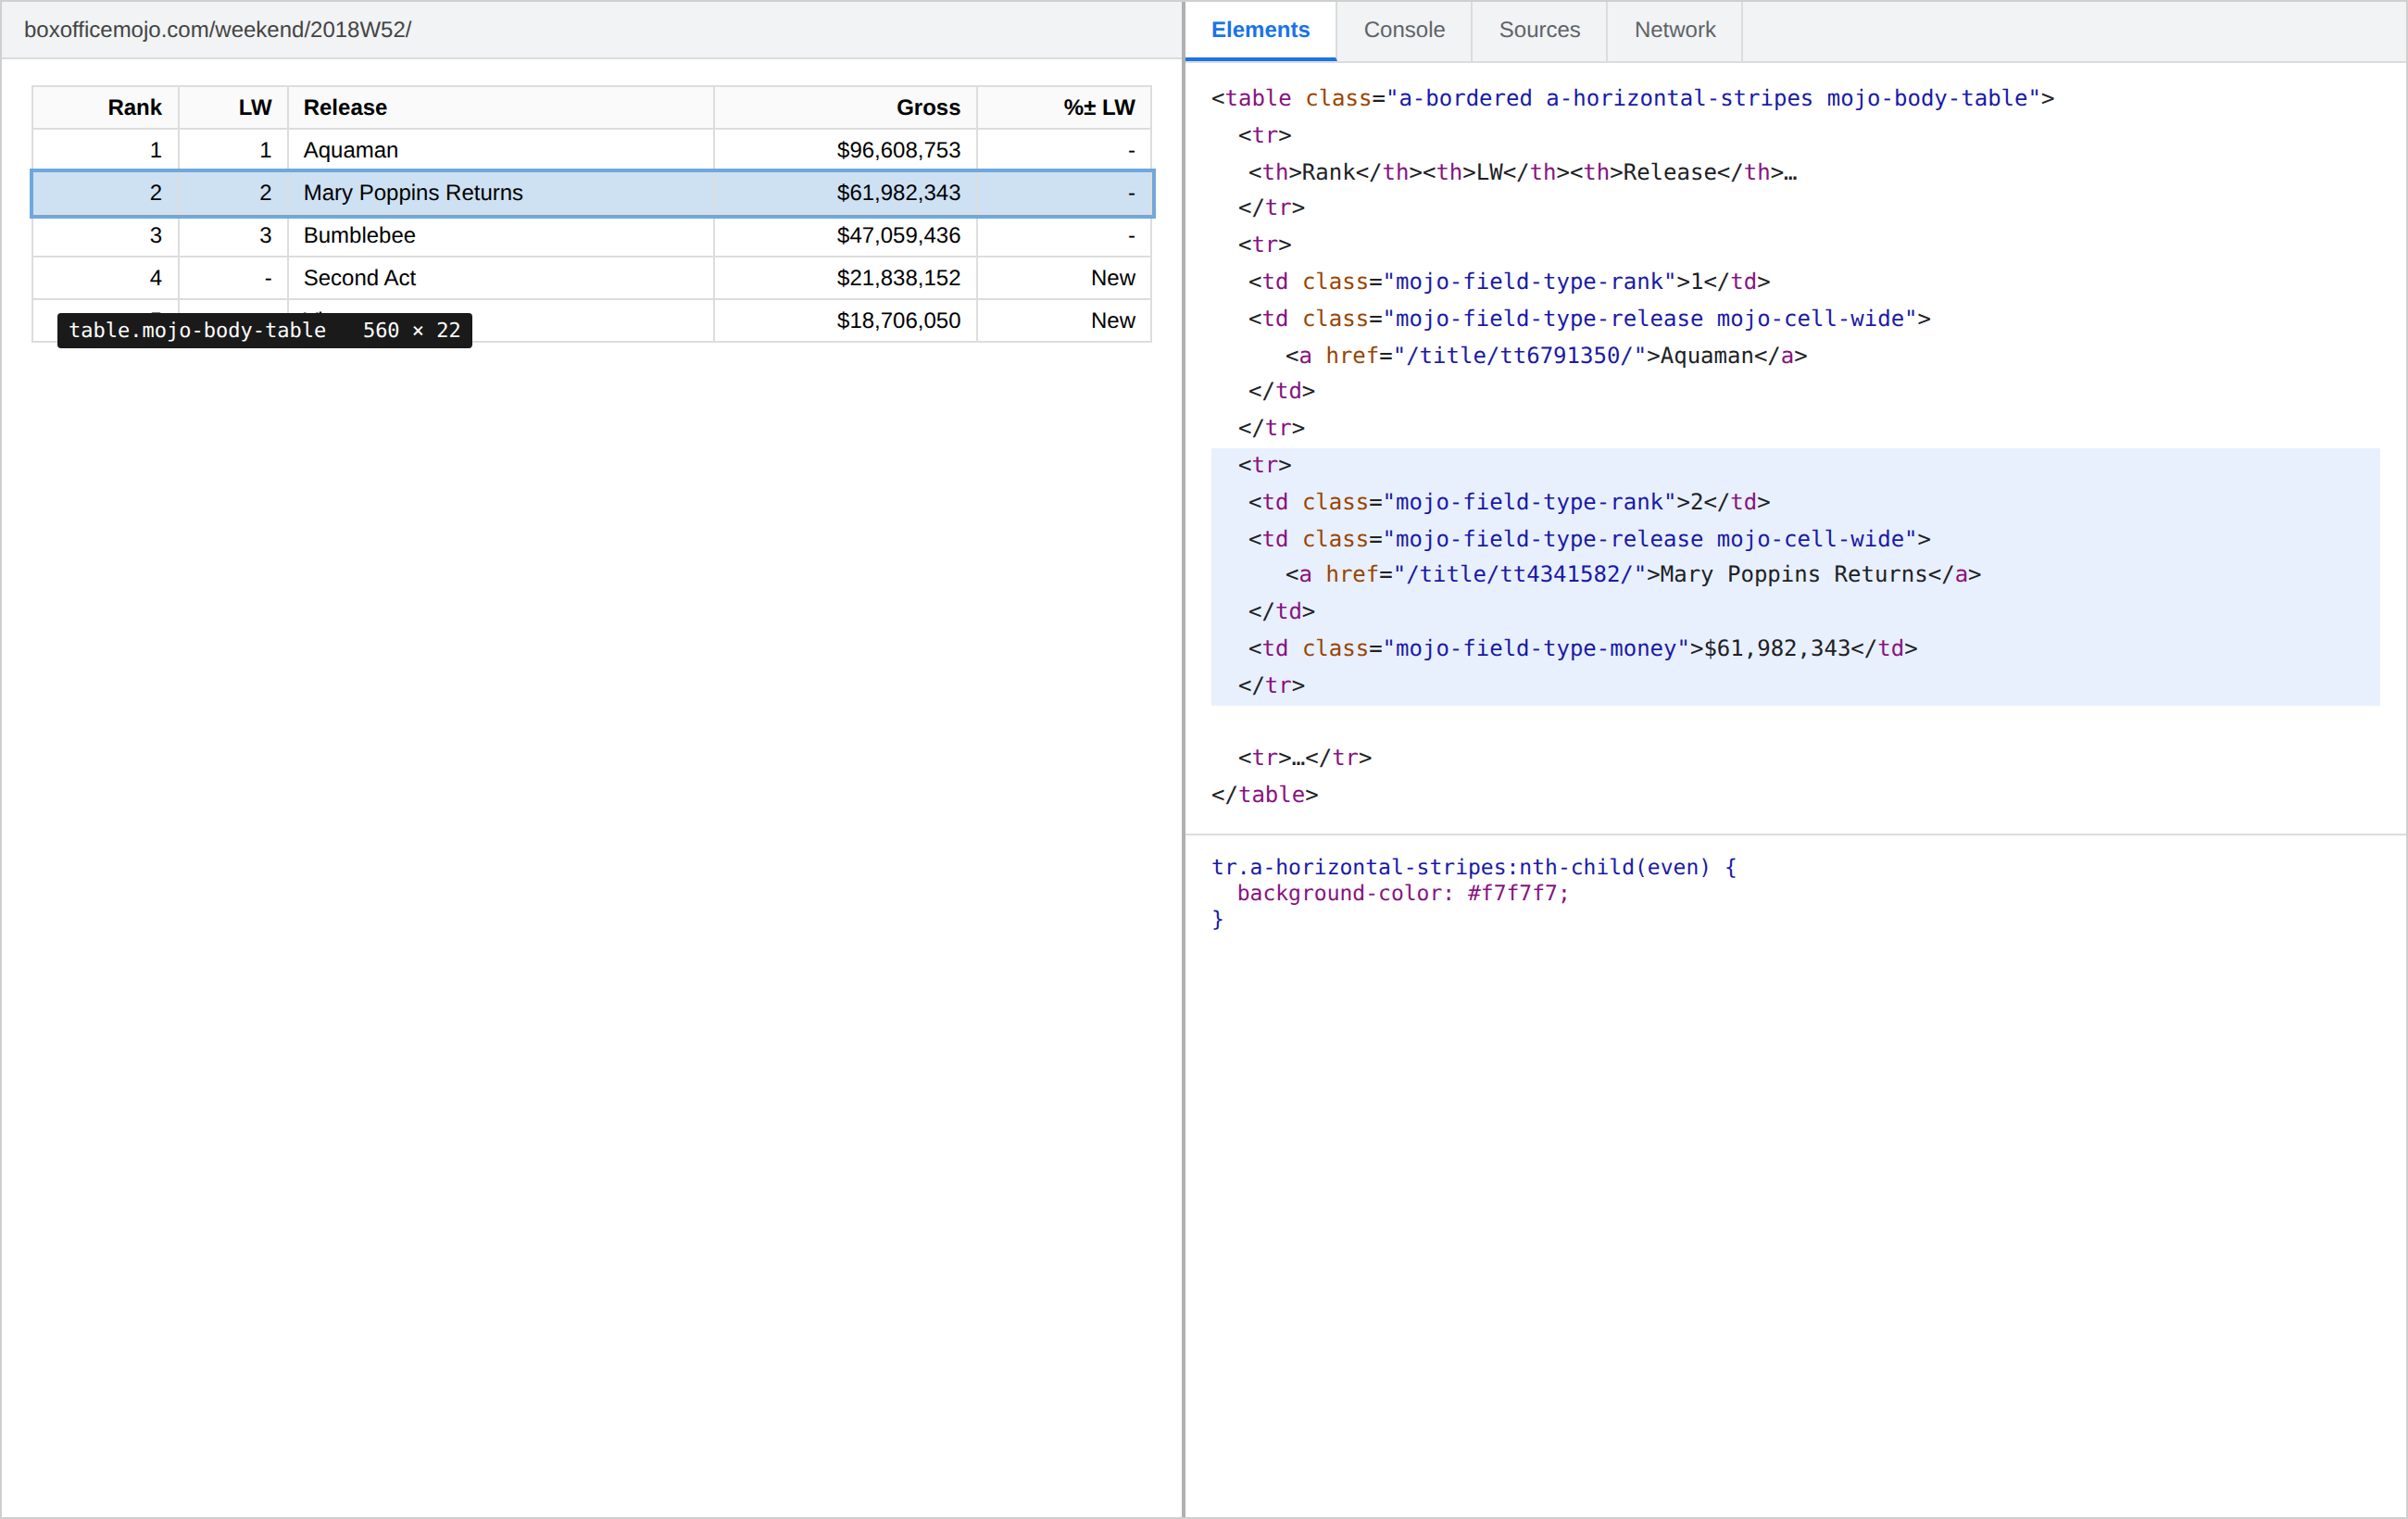
\includegraphics[width=\textwidth]{img/dev_tools_inspect.png}\\
            {\scriptsize Inspect first, code second.}
        \end{column}
    \end{columns}
    \bottomcite{Textbook Ch.~6, ``From HTML to Data.''}
\end{frame}

\begin{frame}{Three strategies, increasingly general}
    \begin{columns}[T]
        \begin{column}{0.58\textwidth}
        \begin{enumerate}
            \item \textbf{Manual table parsing} --- walk \texttt{<table>} $\rightarrow$ \texttt{<tr>} $\rightarrow$ \texttt{<td>} by hand. Most control, most code.
            \vspace{0.5em}
            \item \texttt{\textbf{pandas.read\_html()}} --- one call grabs every table on a page. Least code, least control.
            \vspace{0.5em}
            \item \textbf{Custom parser} --- navigate the DOM tree for data that isn't in a table (\texttt{<div>}s + CSS classes).
        \end{enumerate}

        \vspace{1em}

        Choose the \textit{simplest} strategy that fits the page --- and be ready to fall back to a more general one.
        \end{column}
        \begin{column}{0.38\textwidth}
            \centering
            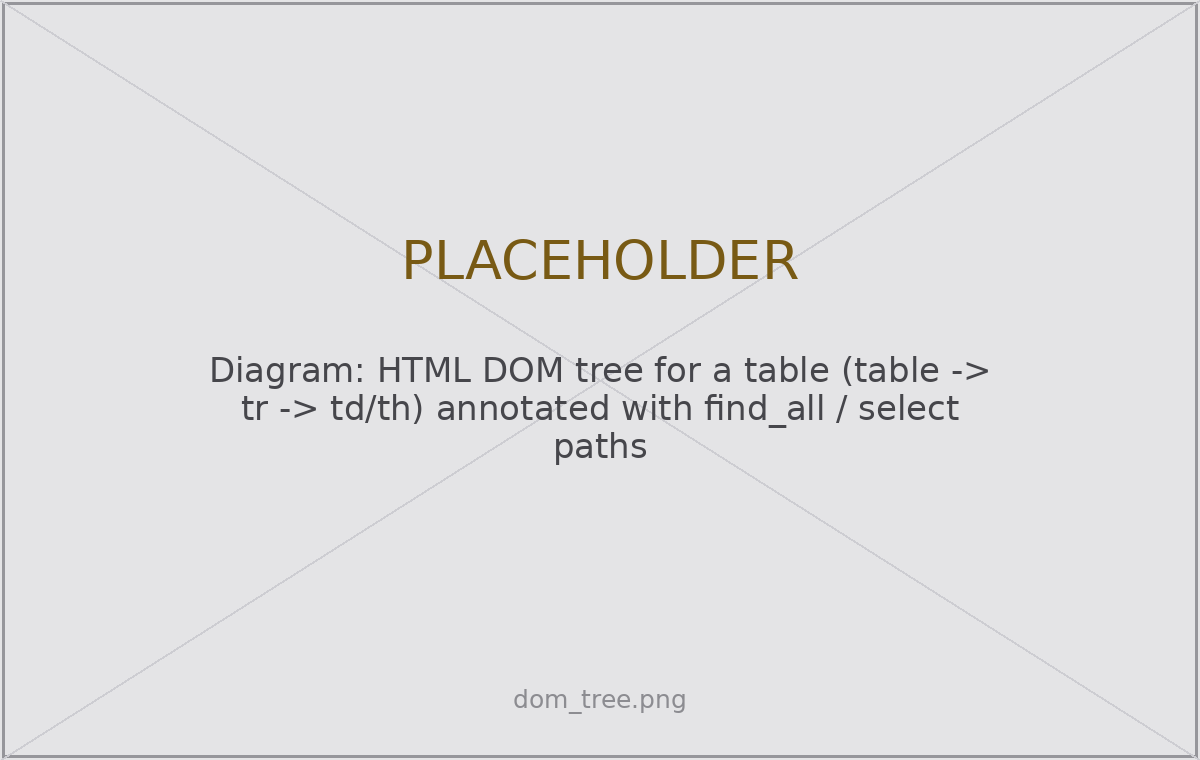
\includegraphics[width=\textwidth]{img/dom_tree.png}
        \end{column}
    \end{columns}
    \bottomcite{Textbook Ch.~6.}
\end{frame}

\begin{frame}{Inspect before you parse}
    \begin{columns}[T]
        \begin{column}{0.5\textwidth}
            Every scrape starts in the browser's developer tools, not in Python.

            \vspace{1em}

            \begin{itemize}
                \item Right-click the data $\rightarrow$ \textbf{Inspect}
                \item Find the \texttt{<table>}, or the repeating \texttt{<div>} container
                \item Note the tags, \texttt{class} names, and \texttt{id}s that anchor your target
                \item ``Copy selector'' gives you a CSS path to paste into \texttt{select()}
            \end{itemize}

            \vspace{1em}

            The page is a \textbf{hypothesis}: inspect, guess an anchor, verify the count, refine.
        \end{column}
        \begin{column}{0.46\textwidth}
            \centering
            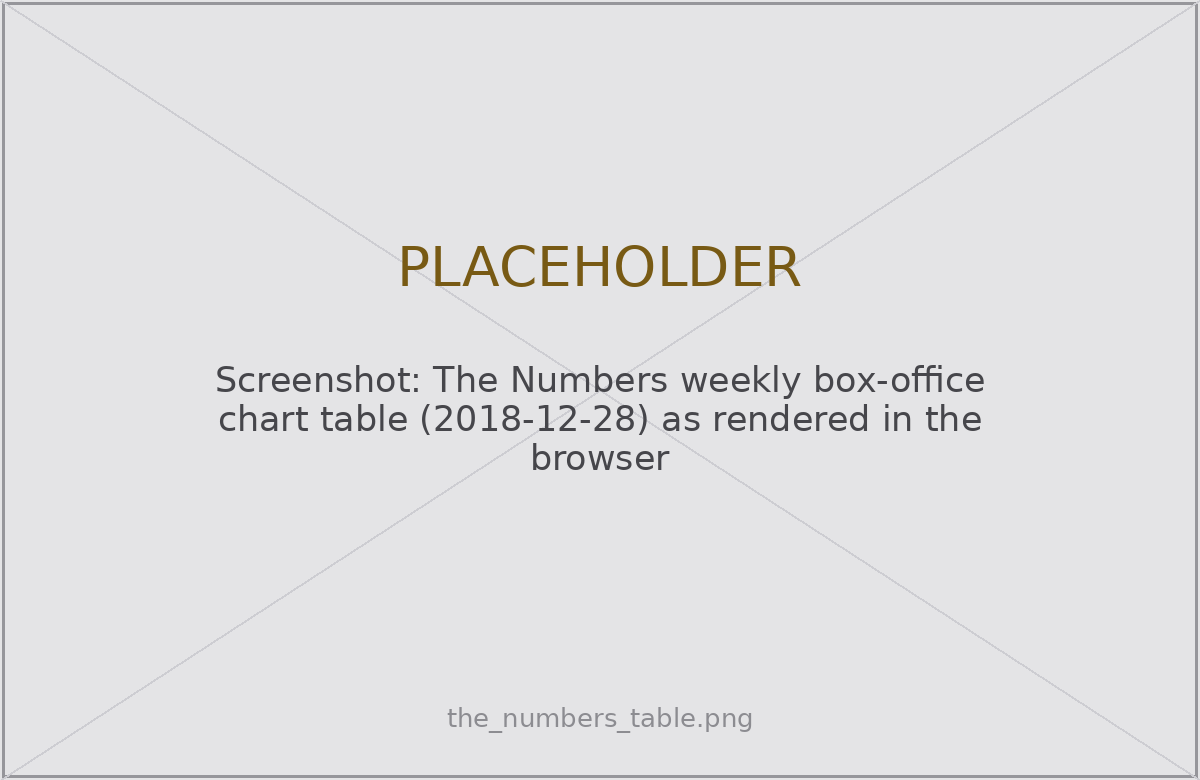
\includegraphics[width=\textwidth]{img/the_numbers_table.png}\\
            {\scriptsize The Numbers weekly box-office chart --- our first target.}
        \end{column}
    \end{columns}
    \bottomcite{Textbook Ch.~6, ``Retrieving and Inspecting.''}
\end{frame}

\begin{frame}{What the notebook covers}
    This week's companion notebook builds one skill at a time:
    \begin{itemize}
        \item \textbf{Strategy 1} --- box-office revenue from The Numbers, cell by cell
        \item \textbf{Strategy 2} --- highest-grossing films from Wikipedia with \texttt{read\_html()} + cleanup
        \item \textbf{Strategy 3} --- Oscar nominees from nested \texttt{<div>}s, then Colorado legislators
        \item \textbf{Reuse} --- abstract a working parser into a function; rate-limit; handle errors
    \end{itemize}

    \vspace{1em}

    \begin{alertblock}{Connecting to Ch.~2 (Ethics)}
        Before pointing a loop at any site, check its \texttt{robots.txt} and Terms of Service, and reuse \texttt{responsible\_get()} from the ethics chapter. Politeness is not optional.
    \end{alertblock}
\end{frame}

% =========================================================================
\section{Wednesday · Notebook Lab}
% =========================================================================

\begin{frame}[fragile]{Strategy 1 --- manual table parsing}
    Retrieve, then find the right table (pages hide data tables among navigation tables):
\begin{lstlisting}
import requests
from bs4 import BeautifulSoup

url = "https://www.the-numbers.com/box-office-chart/weekly/2018/12/28"
headers = {"User-Agent": "WebDataScience/1.0 (you@colorado.edu)"}
soup = BeautifulSoup(requests.get(url, headers=headers).text, "html.parser")

tables = soup.find_all("table")
for i, table in enumerate(tables):          # inspect each candidate
    print(i, len(table.find_all("tr")), "rows")
\end{lstlisting}
    \bottomcite{Textbook Ch.~6, Strategy 1.}
\end{frame}

\begin{frame}[fragile]{The one-line bug that shifts every column}
    \begin{columns}[T]
        \begin{column}{0.52\textwidth}
        Tempting shortcut:
\begin{lstlisting}
# DON'T: silently drops empty cells
row.text.split("\n")
\end{lstlisting}
        Correct --- walk cell by cell so \textbf{empty cells stay aligned}:
\begin{lstlisting}
cells = row.find_all(["td", "th"])
values = [c.get_text(strip=True)
          for c in cells]
\end{lstlisting}
        \end{column}
        \begin{column}{0.44\textwidth}
            A blank header cell (the ``previous rank'' column) is easy to lose.

            \vspace{0.75em}

            Split-on-newline drops it --- and every value after shifts one column left, so \textbf{Movie} quietly fills with distributor names.

            \vspace{0.75em}

            The extra line of code buys correctness.
        \end{column}
    \end{columns}
    \bottomcite{Textbook Ch.~6, ``Extracting Row Data.''}
\end{frame}

\begin{frame}[fragile]{Strategy 2 --- \texttt{pandas.read\_html()}}
\begin{lstlisting}
import pandas as pd

url = "https://en.wikipedia.org/wiki/2018_in_film"
tables = pd.read_html(url)          # every table on the page -> list of DataFrames
films = pd.read_html(url, header=0)[3]   # pick the right one by index
\end{lstlisting}
    Powerful, but rarely perfect. Expect to spend as long \textbf{cleaning} as extracting:
\begin{lstlisting}
df = df[df.iloc[:, 0] != df.columns[0]]              # drop repeated header rows
df.columns = [c.strip().lower().replace(" ", "_") for c in df.columns]
df["worldwide_gross"] = pd.to_numeric(               # "$1,234" -> 1234
    df["worldwide_gross"].str.replace(r"[\$,]", "", regex=True), errors="coerce")
df["studio"] = df["studio"].ffill()                  # fill merged (colspan) cells
\end{lstlisting}
    \bottomcite{Textbook Ch.~6, Strategy 2. \texttt{errors="coerce"} keeps the pipeline alive on bad cells.}
\end{frame}

\begin{frame}[fragile]{Strategy 3 --- custom parser \& CSS selectors}
    Non-tabular data (Oscar nominees) lives in nested \texttt{<div>}s. Find a reliable anchor, then search within it --- \texttt{find()} + \texttt{find\_all()}, or one CSS selector:
\begin{lstlisting}
# navigate: up to a unique parent, then down to the repeating rows
area = soup.find("div", class_="field--name-field-award-categories")
categories = area.find_all("div", class_="view-grouping") if area else []

# equivalent, in one readable line (paste from "Copy selector"):
soup.select("div.field--name-field-award-categories div.view-grouping")
\end{lstlisting}
    \begin{columns}[T]
        \begin{column}{0.6\textwidth}
            \texttt{select()} returns a list like \texttt{find\_all()}; \texttt{select\_one()} returns one like \texttt{find()}.
        \end{column}
        \begin{column}{0.36\textwidth}
            \centering
            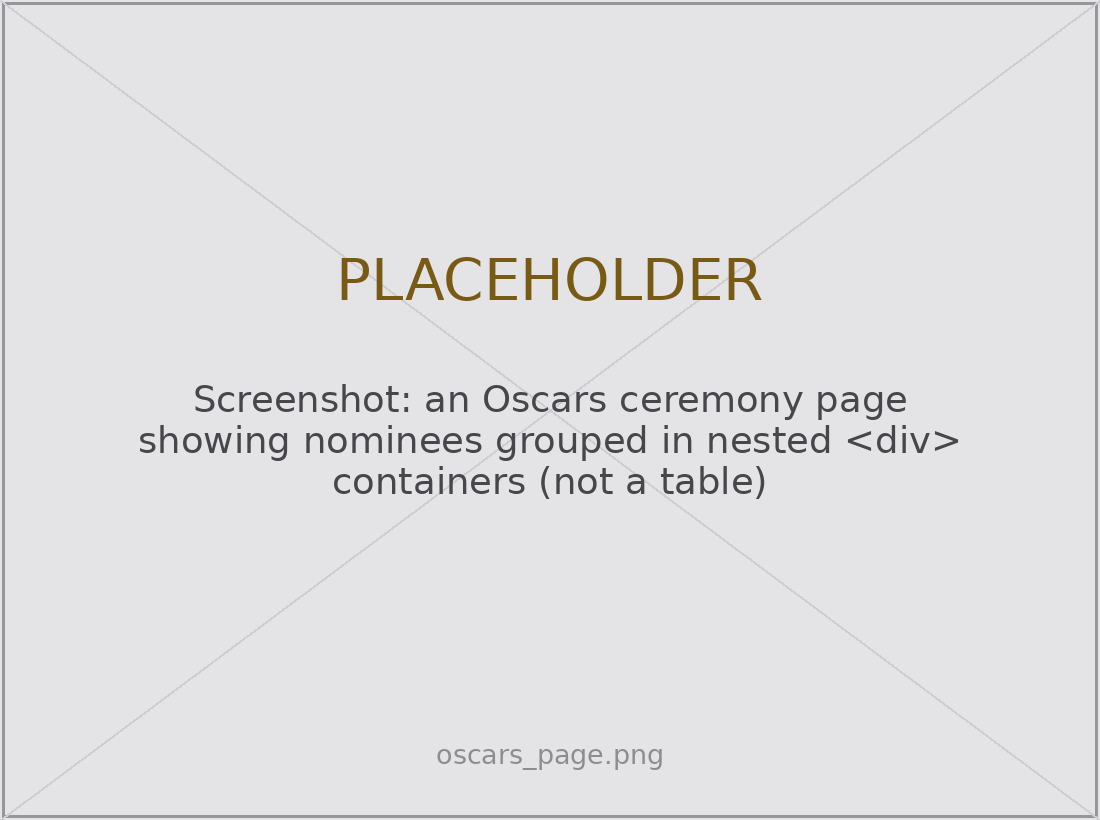
\includegraphics[width=\textwidth]{img/oscars_page.png}
        \end{column}
    \end{columns}
    \bottomcite{Textbook Ch.~6, Strategy 3.}
\end{frame}

\begin{frame}[fragile]{Make it reusable --- and defensive}
    Abstract the working parser into a function; keep the \texttt{sleep} in the \textit{caller}, not the function:
\begin{lstlisting}
for year in range(2020, 2025):
    df = scrape_oscar_year(year, headers)   # returns empty DataFrame on failure
    all_years.append(df)
    time.sleep(1)                           # politeness lives in the loop
\end{lstlisting}
    Wrap fragile parsing so one bad page doesn't kill the run:
\begin{lstlisting}
try:
    response.raise_for_status()
except requests.RequestException as e:
    print(f"Request failed: {e}"); return None
# AttributeError fires when .find() returns None and you call .text on it
# -- the single most common scraping error.
\end{lstlisting}
    \bottomcite{Textbook Ch.~6, ``Abstracting into Functions'' \& ``Error Handling Patterns.''}
\end{frame}

\begin{frame}{Lab: work these, then show-and-tell}
    \begin{columns}[T]
        \begin{column}{0.62\textwidth}
            Work through the notebook exercises in pairs:
            \begin{enumerate}\small
                \item Wikipedia table via \texttt{read\_html} + a visualization
                \item Custom parser for a non-tabular page (document your selectors)
                \item Extend it to multiple pages (sleep, try/except, a function)
                \item Non-English Wikipedia --- what encoding cleanup is needed?
                \item Cache-first: download once to \texttt{cache/}, parse offline
                \item[6.] \textcolor{tab-purple}{\textbf{5617}}: audit two sites' ToS \& \texttt{robots.txt} vs.\ \textcite{fiesler2020no}
            \end{enumerate}
        \end{column}
        \begin{column}{0.34\textwidth}
            \begin{block}{Show-and-Tell}
                \footnotesize Come ready to share:
                \begin{itemize}\footnotesize
                    \item a challenging bug
                    \item interesting data you pulled
                    \item a provocation for a research design
                \end{itemize}
            \end{block}
        \end{column}
    \end{columns}
\end{frame}

\begin{frame}[standout]
    Sites redesign without warning.\\
    When a parser breaks, that's not a bug in your code ---\\
    it's the web working as designed.\\[1em]
    {\large Re-inspect, re-hypothesize, re-verify.}
\end{frame}

% =========================================================================
\section{Friday · Textbook Revisions}
% =========================================================================

\begin{frame}{Improving Chapter 6 together}
    \begin{columns}[T]
        \begin{column}{0.6\textwidth}
            Today we make the book better. Each of you opens a \textbf{pull request} against \texttt{ch-06-static-pages.qmd} and reviews a classmate's.

            \vspace{1em}

            The workflow (from Week 1):
            \begin{enumerate}\small
                \item Branch / fork the book repo
                \item Edit the chapter; commit with a clear message
                \item Open a PR describing \textit{what} and \textit{why}
                \item Review two peers' PRs: kind, specific, actionable
            \end{enumerate}
        \end{column}
        \begin{column}{0.36\textwidth}
            \centering
            
\includegraphics[width=\textwidth]{img/pr_review.png}
        \end{column}
    \end{columns}
    \bottomcite{Contributions \& reviews count toward the Textbook Revisions grade (30\%).}
\end{frame}

\begin{frame}{A revision menu for Chapter 6}
    High-value targets --- pick one and scope it to a single PR:
    \begin{itemize}
        \item \textbf{Test the code against live sites.} The Numbers, Wikipedia, and Oscars pages drift. Run the notebook, report what broke, and fix the selectors (this is the chapter's own ``A Note on Fragility'').
        \item \textbf{Close a gap in ``Common Issues to Debug.''} Add a worked \texttt{\textbackslash xa0} / non-breaking-space example, or a \texttt{colspan}/\texttt{rowspan} case \texttt{read\_html} mishandles.
        \item \textbf{Add a figure.} A clean DOM-tree diagram, or an annotated Inspector screenshot, would help Strategy 1 and 3.
        \item \textbf{Strengthen an exercise.} Add expected output, a rubric, or a starter cell so exercises are self-checking.
        \item \textbf{Extend ``Further Reading.''} A data-journalism scrape (ProPublica, The Markup) tied to the ``Public Interest'' callout.
    \end{itemize}
    \bottomcite{Targets drawn from the chapter's callouts, ``Common Issues,'' and ``Further Reading.''}
\end{frame}

\begin{frame}{What makes a good revision \& a good review}
    \begin{columns}[T]
        \begin{column}{0.48\textwidth}
            \begin{block}{A strong PR}
                \begin{itemize}\small
                    \item One focused change, clearly titled
                    \item Explains the problem it fixes
                    \item Builds (\texttt{quarto render}) without errors
                    \item Matches the book's voice and notation
                    \item Discloses any AI assistance
                \end{itemize}
            \end{block}
        \end{column}
        \begin{column}{0.48\textwidth}
            \begin{block}{A strong review}
                \begin{itemize}\small
                    \item Runs / reads the change, not just skims
                    \item Names specifics (line, claim, code)
                    \item Separates ``must fix'' from ``nice to have''
                    \item Is generous --- assume good faith
                    \item Ends with a clear verdict
                \end{itemize}
            \end{block}
        \end{column}
    \end{columns}
    \vspace{0.5em}
    \centering\small Next week: \textbf{Archived web pages} --- scraping the past with the Wayback Machine.
\end{frame}

% =========================================================================
\begin{frame}{Key takeaways}
    \begin{enumerate}
        \item Scraping is a pipeline: \textbf{retrieve $\rightarrow$ inspect $\rightarrow$ anchor $\rightarrow$ extract $\rightarrow$ DataFrame}.
        \item Start with \texttt{read\_html()} for tables; fall back to manual or custom parsing for control.
        \item Navigate cell by cell --- shortcuts silently misalign columns.
        \item Abstract into functions, rate-limit in the loop, and code defensively.
        \item Pages change: the durable skill is \textbf{inspect, hypothesize, verify} --- not memorized class names.
    \end{enumerate}
    \vspace{1em}
    \bottomcite{Reading: Textbook Ch.~6. Related: \textcite{mitchell2018web}; \textcite{vandenbroucke2018practical}.}
\end{frame}

\end{document}
